\section{Utilisation par l'homme}

	\subsection{Usage culinaire}

Toutes les grenouilles ne sont pas comestibles. 
Certaines espèces sont même toxiques et d'autres sont des espèces menacées de disparition dont les populations sont désormais protégées.

En cuisine française, ce sont les cuisses qui sont consommées. 
Les Français ont la réputation mondiale d'être des mangeurs de grenouilles, ce qui leur a valu leur surnom anglais de froggies, frog signifiant grenouille en anglais. 
Ainsi, on appelle $\ll$ Vallée des grenouilles $\gg$ un quartier de Londres, peuplé de beaucoup de Français.
En Italie les Français sont parfois appelés les mangiarane, c'est-à-dire les $\ll$ mangeurs de grenouilles $\gg$.

Traditionnellement, il s'agissait d'espèces locales, comme les grenouilles rousses (Rana temporaria) et vertes (Rana esculenta) désormais protégées à l'état sauvage en France, mais encore disponibles dans de rares élevages agréés. 
Elles ont été remplacées par des grenouilles asiatiques : Rana tigrina, Rana crassa et Rana catesbeiana quand elles sont surgelées et Rana ridibunda pour les importations vivantes.
D'autres pays d'Europe ou les États-Unis consomment également ces grenouilles d'importation.

Les autochtones au Cameroun mangent couramment Trichobatrachus robustus : chassé avec de longues lances, des machettes, et même parfois des armes à feu pour éviter ses griffes rétractiles, il finit alors au menu, rôti (entier). 
Dans les monts Rumpi, zone protégée à l'ouest du Cameroun, les autochtones en mangent les têtards, qui seraient assez gros.

\begin{figure}
	
	\begin{center}
		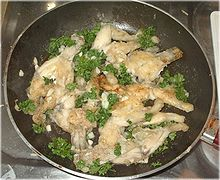
\includegraphics[scale=1]{cuisine/miam.JPG}
			\caption{Cuisses de grenouilles}
			\label{fig:gre}
	\end{center}

\end{figure}

\subsection{Animal de laboratoire}

La grenouille est l'un des animaux utilisés couramment dans l'enseignement pour étudier par la dissection le système nerveux, l'appareil digestif ou l'appareil uro-génital.

Les espèces du genre Xenopus, qui ont pour certaines la rare particularité pour un animal d'être polyploïdes, sont utilisées comme modèle en laboratoire, notamment dans l'étude de l'embryogénèse et génétique du développement. 

\subsection{Animal de compagnie}

La grenouille fait partie des nouveaux animaux de compagnie (NAC).

On a par ailleurs relevé un cas d'apprivoisement de grenouille sauvage à Meudon au XIXe siècle ; il est détaillé par le naturaliste Louis Eugène Robert.

    « Je croyais n'avoir rien à signaler en erpétologie ; cependant l'apprivoisement bien constaté d'une grenouille est un fait trop intéressant pour le passer sous silence. Voici un extrait de ce que M. Guérin Méneville, zoologue des plus distingués, a bien voulu me communiquer à ce sujet :
    « Nous n'avions jamais entendu dire que la grenouille fût susceptible de s'apprivoiser, de venir à la voix, de se laisser toucher, de prendre de la mie de pain, quoique jouissant toujours de la plus complète liberté dans un grand bassin, en compagnie d'autres grenouilles et de nombreux poissons de la Chine ; c'est cependant ce que j'ai été à même de voir un grand nombre de fois, ainsi que beaucoup d'autres personnes.
    « Lorsque madame Panckoucke, dont l'amabilité ne le cède en rien au mérite de l'artiste-peintre, assistait au déjeuner de ses poissons dorés, une belle grenouille verte ne tardait pas à paraître et à se pavaner au milieu d'eux, en cherchant à leur disputer quelques miettes. Madame Ernestine P....... l'appelait-elle doucement, la batracienne venait au bord du bassin, y appuyait ses pattes de devant, et attendait qu'on voulût bien lui donner un peu de mie trempée ; elle se laissait alors toucher et caresser par les dames dans les mains desquelles elle se glissait volontiers ; enfin, on pouvait la sortir de l'eau et la transporter assez loin sans qu'elle parût s'inquiéter ni chercher à fuir. »

— Louis Eugène Robert, Histoire et description naturelle de la commune de Meudon, 1843
